\newpage

\chapter{Sprint 2: Equipment Monitoring and Inventory}

\cfoot{\thepage}

\parindent=0.5in
\onehalfspacing

\section{Introduction}

Sprint 2, titled "Equipment Monitoring and Inventory," extends the site management foundation established in Sprint 1 by introducing comprehensive equipment tracking and inventory management capabilities. This sprint addresses user stories US-005A-C (Equipment CRUD operations), US-006 (Equipment Status Monitoring), and US-016A-B (Equipment Types and Maintenance Rules) from Chapter 2's product backlog.

The sprint focuses on enabling network engineers and technicians to monitor all network hardware across telecommunications sites, managing equipment lifecycle from installation through warranty expiration, tracking real-time status changes, and maintaining accurate records critical for proactive network maintenance. This capability directly supports the operational requirements identified in Chapter 2's stakeholder analysis for Network Engineers and Field Technicians.

\section{Sprint Backlog}

During sprint planning, we defined the tasks required for Sprint 2 implementation. Table 4.1 presents the sprint backlog with user stories, tasks, complexity assessments, and effort estimates.

\begin{table}[H]
\centering
\small
\begin{tabular}{|p{2.5cm}|p{4cm}|p{3.2cm}|p{2.2cm}|p{1.5cm}|}
\hline
\textbf{Functionality} & \textbf{User Story} & \textbf{Tasks} & \textbf{Complexity} & \textbf{Estimate} \\
\hline

\multirow{3}{2.5cm}{Add Equipment (US-005A)} & 
\multirow{3}{4cm}{As admin or engineer, I can add new equipment with serial numbers}
& Equipment creation logic & Medium & 5 \\
\cline{3-5}
& & Serial number validation & Hard & 5 \\
\cline{3-5}
& & Integration and testing & Medium & 3 \\
\hline

\multirow{3}{2.5cm}{Edit Equipment (US-005B)} & 
\multirow{3}{4cm}{As admin or engineer, I can edit equipment details and specifications}
& Equipment update logic & Medium & 4 \\
\cline{3-5}
& & Edit modal interface & Easy & 2 \\
\cline{3-5}
& & Validation and testing & Medium & 3 \\
\hline

\multirow{3}{2.5cm}{Delete Equipment (US-005C)} & 
\multirow{3}{4cm}{As admin, I can delete obsolete equipment from inventory}
& Equipment deletion logic & Easy & 2 \\
\cline{3-5}
& & Confirmation dialog & Easy & 1 \\
\cline{3-5}
& & Cascade testing & Medium & 3 \\
\hline

\multirow{3}{2.5cm}{Status Monitoring (US-006)} & 
\multirow{3}{4cm}{As all users, I can view equipment status and performance metrics}
& Status tracking logic & Medium & 4 \\
\cline{3-5}
& & Status update interface & Easy & 2 \\
\cline{3-5}
& & Real-time updates & Hard & 4 \\
\hline

\multirow{3}{2.5cm}{Equipment Types (US-016A)} & 
\multirow{3}{4cm}{As admin, I can define equipment type categories for standardization}
& Equipment type system & Medium & 3 \\
\cline{3-5}
& & Type validation & Easy & 2 \\
\cline{3-5}
& & Testing and integration & Medium & 2 \\
\hline

\multirow{3}{2.5cm}{Equipment Statistics} & 
\multirow{3}{4cm}{As manager, engineer, and admin, I can view equipment statistics and metrics}
& Statistics calculation & Medium & 4 \\
\cline{3-5}
& & Dashboard cards design & Easy & 2 \\
\cline{3-5}
& & Testing and validation & Medium & 3 \\
\hline

\end{tabular}
\caption{Sprint 2 Backlog with Task Breakdown}
\label{tab:sprint2_backlog}
\end{table}

The backlog totals 54 story points across six major functionalities. Serial number validation complexity stems from uniqueness enforcement requirements. Real-time status updates require WebSocket implementation for immediate propagation across user sessions.

\section{Conceptual Design}

This section presents the conceptual design models guiding Sprint 2 implementation.

\subsection{Class Diagram}

Figure 4.1 presents the class diagram focusing on equipment management and relationships with telecommunications sites established in Sprint 1.

\begin{figure}[H]
    \centering
    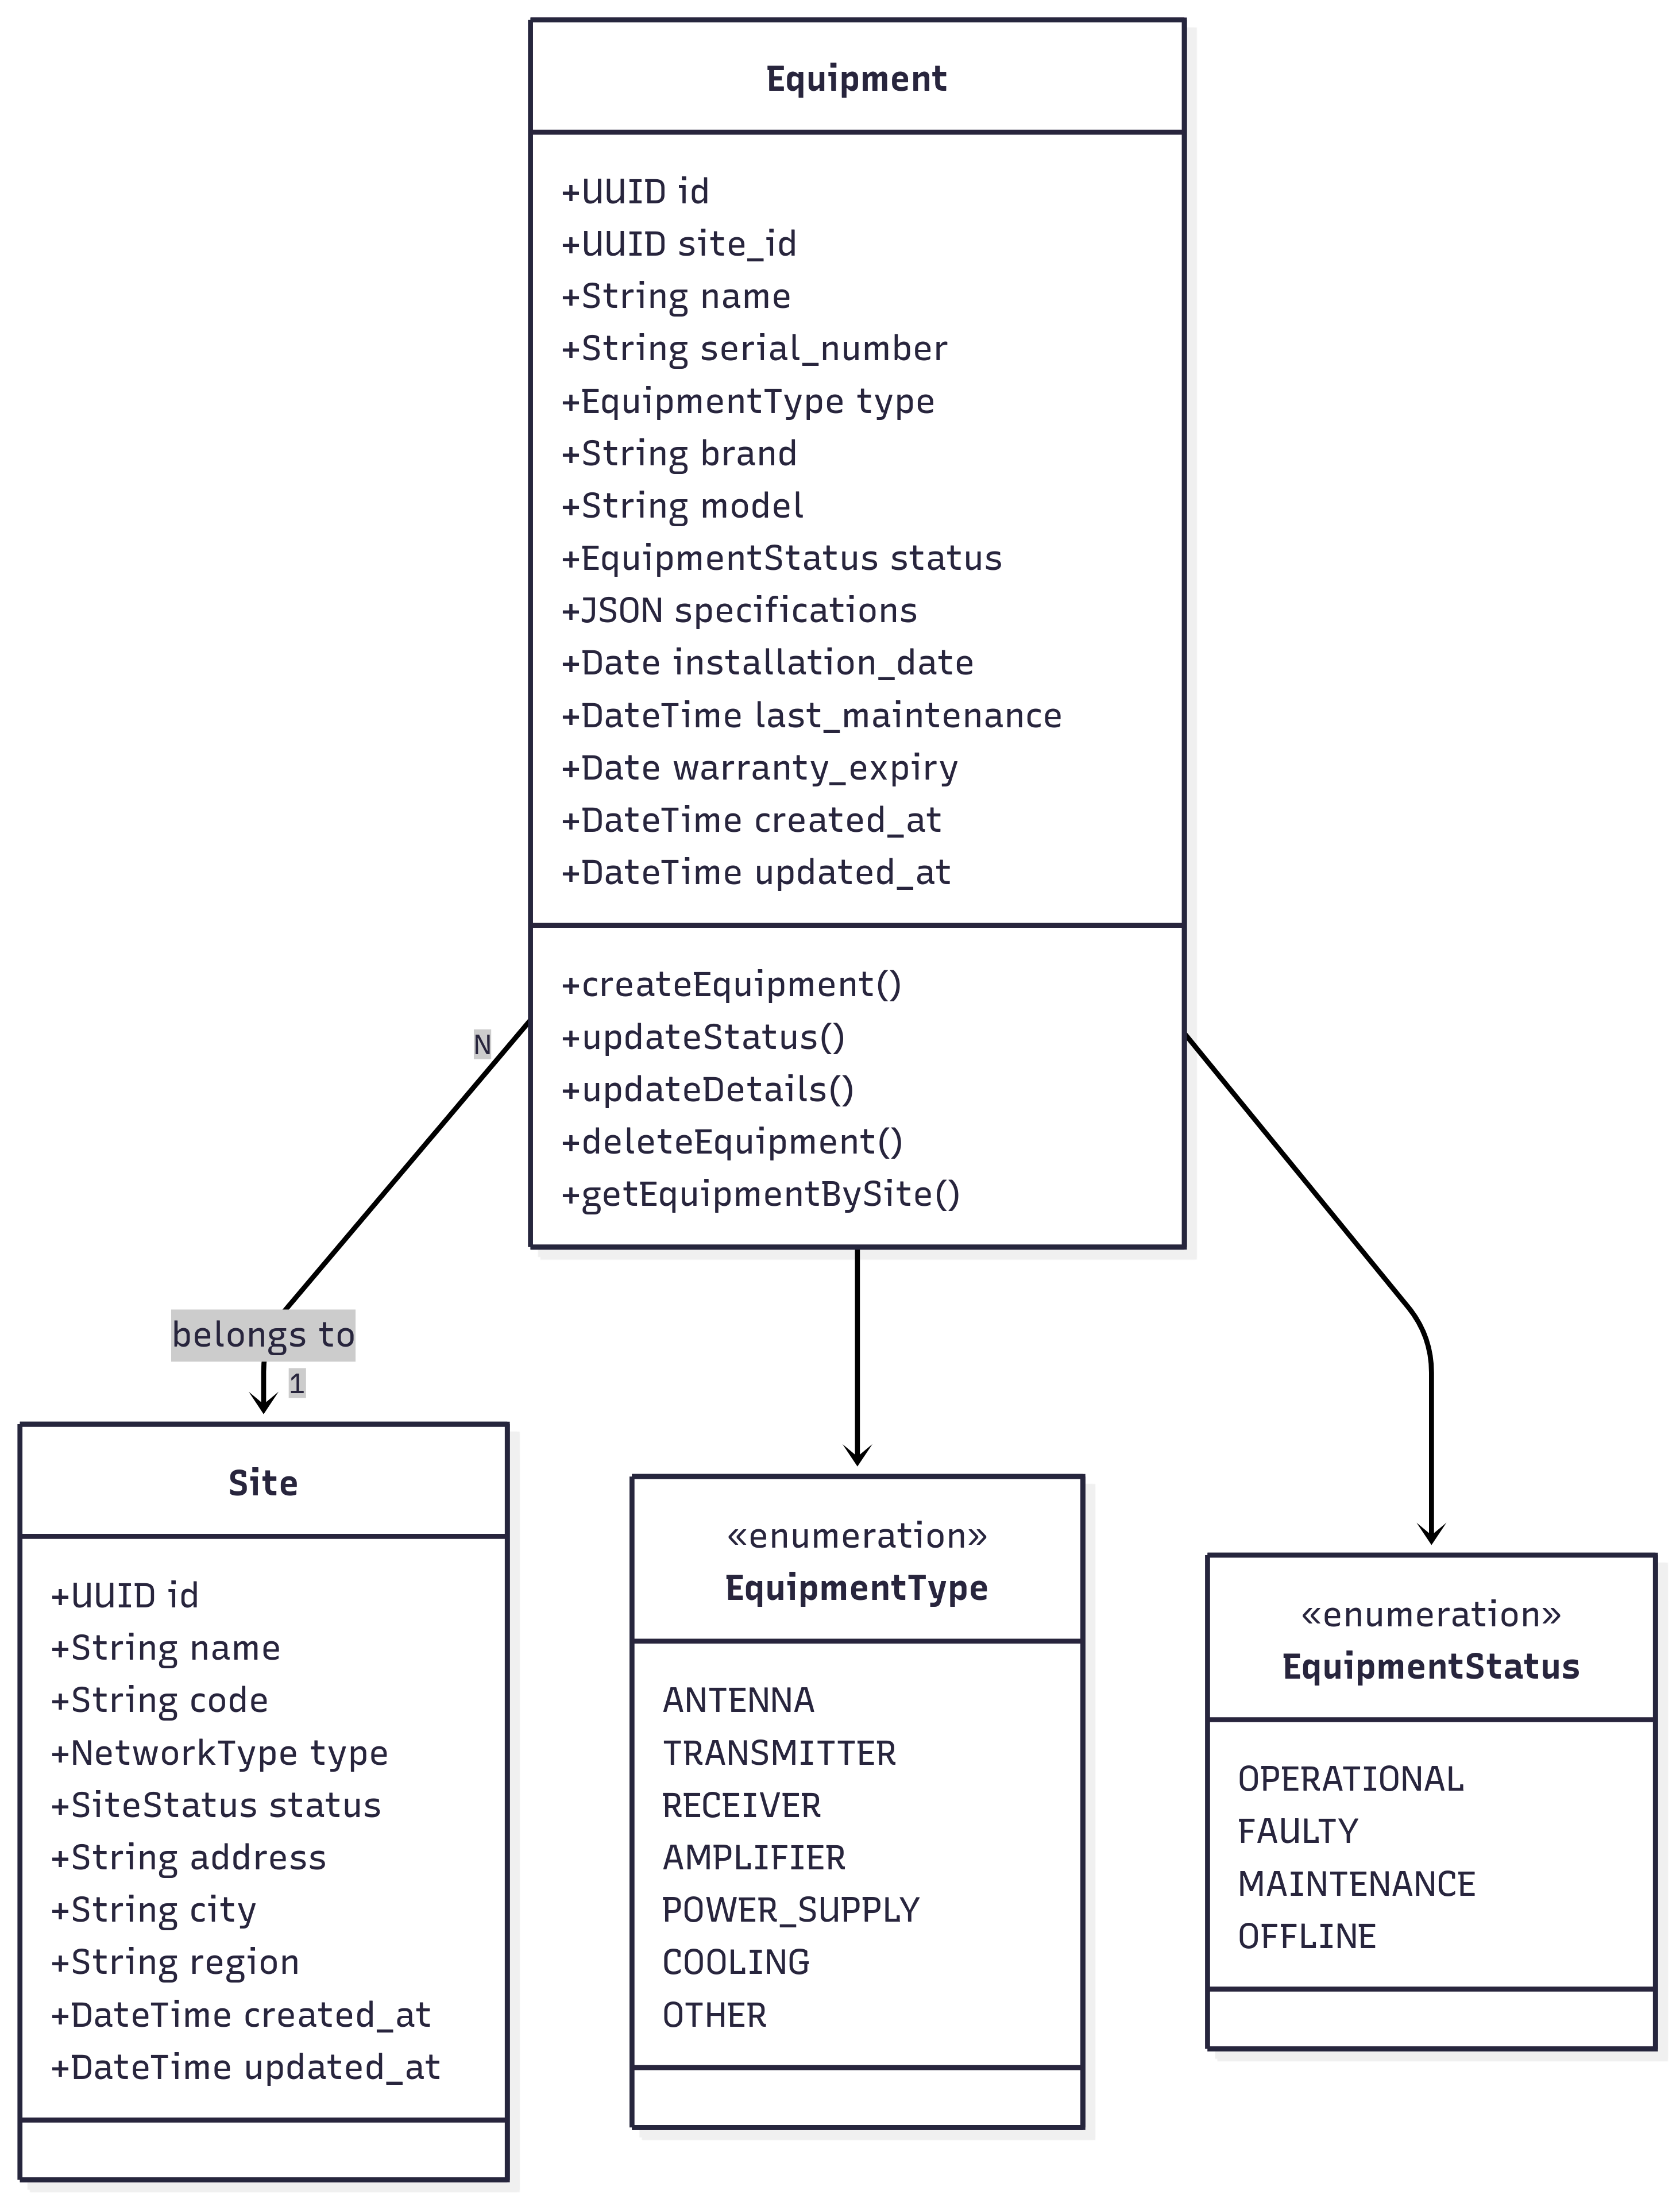
\includegraphics[width=0.95\linewidth]{img/chap_04/equipment_class_diagram.png}
    \caption{Class Diagram - Equipment Monitoring and Inventory}
    \label{fig:class_diagram_sprint2}
\end{figure}


The class diagram (Figure 4.1) illustrates the Equipment entity with attributes following UML standard notation (name : type format). The Equipment class maintains unique serial numbers ensuring equipment traceability, equipment type classifications (antenna, transmitter, receiver, amplifier, power supply, cooling), operational status tracking (operational, faulty, maintenance, offline), brand and model information for vendor management, warranty details with expiration tracking, and installation dates for lifecycle analysis. The many-to-one relationship with Sites ensures every equipment item associates with a specific network location, supporting geographical equipment distribution analysis.

\subsection{Use Case Diagram}

Figure 4.2 presents the use case diagram showing actors and their hierarchical interactions with the equipment management system.

\begin{figure}[H]
    \centering
    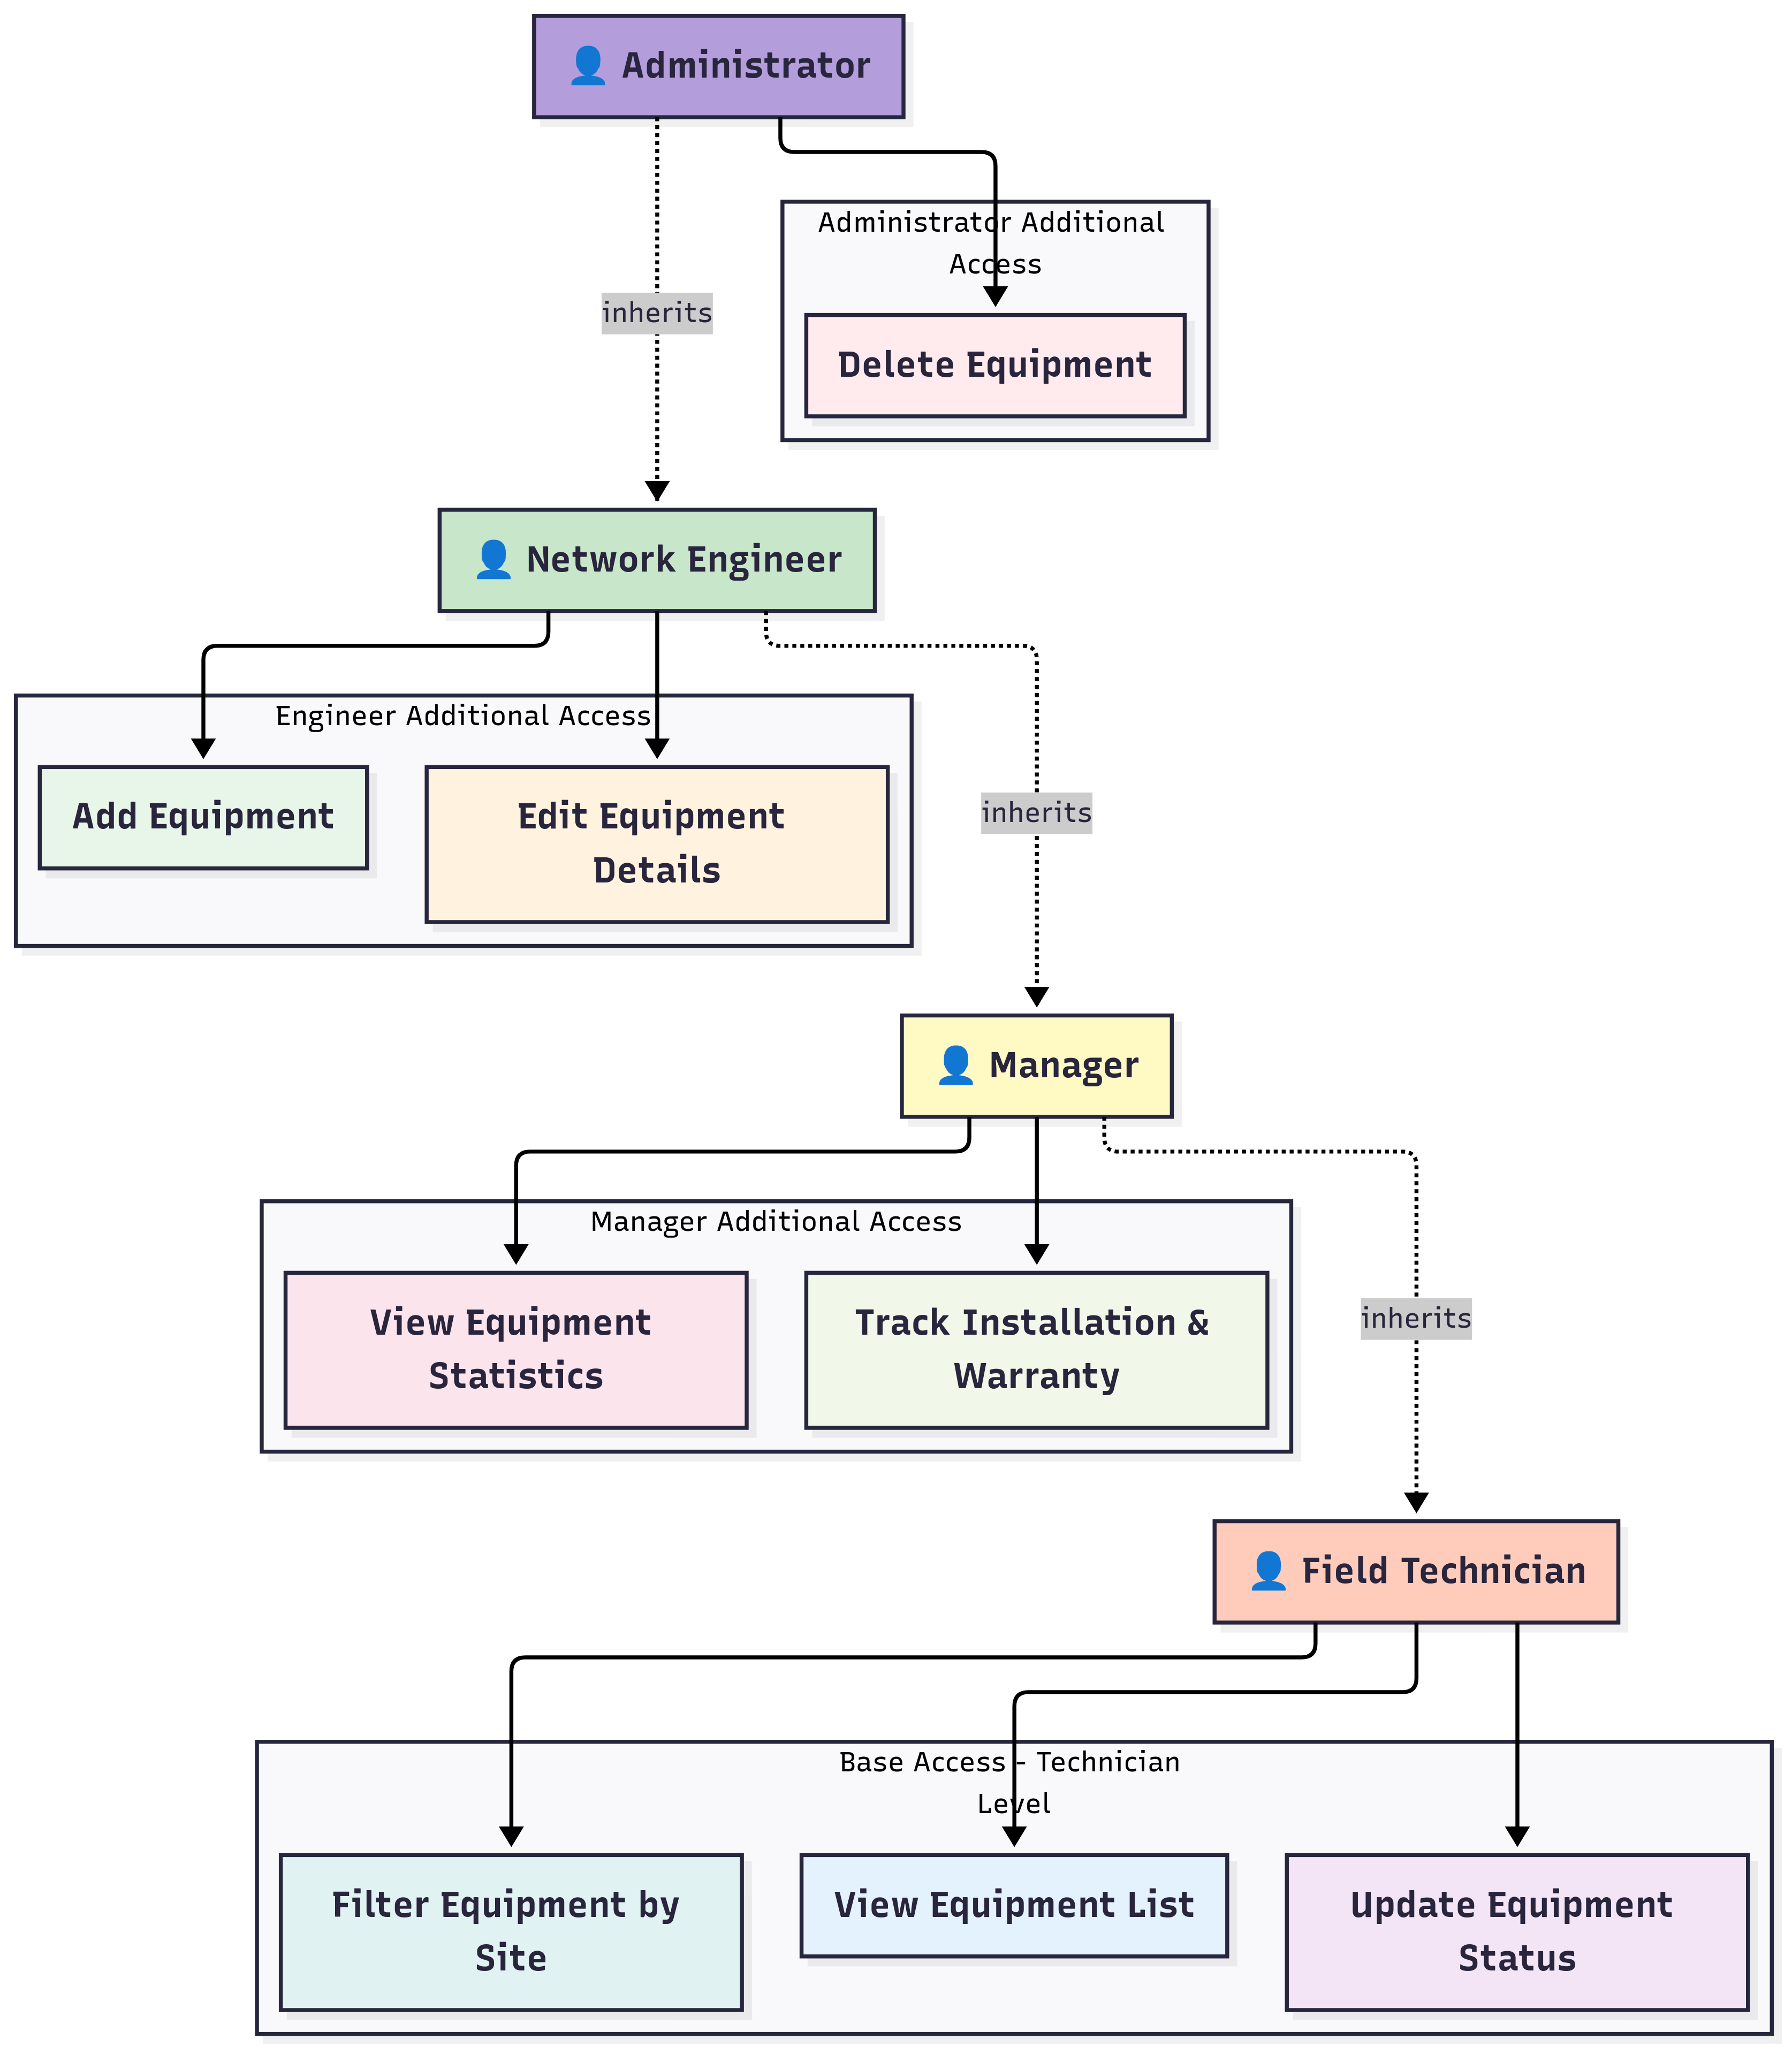
\includegraphics[width=0.85\linewidth]{img/chap_04/equipment_usecase_diagram.png}
    \caption{Use Case Diagram - Equipment Monitoring and Inventory}
    \label{fig:use_case_diagram_sprint2}
\end{figure}

The use case diagram (Figure 4.2) implements an inheritance hierarchy across four actor types reflecting the stakeholder permissions from Chapter 2. Field Technicians possess base access capabilities including viewing equipment lists, updating equipment status after field operations, and filtering equipment by site location. Managers inherit all technician permissions while adding supervisory capabilities including viewing equipment statistics for operational oversight and tracking installation and warranty information for budget planning. Network Engineers inherit all manager permissions while adding technical management capabilities including adding new equipment to inventory and editing equipment details and specifications. Administrators inherit all engineer permissions while possessing exclusive equipment deletion rights for complete lifecycle management.

\textbf{Use Case Description: Add Equipment}

Since equipment CRUD operations share similar processing patterns, we provide detailed information on the "Add Equipment" use case as representative of equipment management functionality. Table 4.2 presents the detailed textual description.

\begin{table}[H]
\centering
\small
\begin{tabular}{|p{3cm}|p{8.5cm}|}
\hline
\textbf{Use Case} & Add Equipment \\
\hline
\textbf{Primary Actors} & Administrator, Network Engineer \\
\hline
\textbf{Pre-condition} & User authenticated with appropriate role; at least one active site exists \\
\hline
\textbf{Post-condition} & Equipment created in database with operational status and unique serial number \\
\hline
\textbf{Main Scenario} & 
1. User accesses equipment management interface
2. User clicks "Add Equipment" button displaying creation modal
3. User fills form: name, serial number, type, brand, model, site assignment
4. User submits form
5. System validates required fields and serial number format
6. System checks serial number uniqueness via database query
7. System verifies user permissions via Row Level Security
8. System creates equipment record with "operational" default status
9. System updates equipment list in real-time
10. System displays success confirmation
\\
\hline
\textbf{Exception Scenarios} & 
E1: Missing required fields → Display field-specific error messages
E2: Duplicate serial number → Display "Serial number already exists"
E3: Invalid equipment type → Display "Invalid equipment type selected"
E4: Insufficient permissions → Display access denied error
E5: Server connection problem → Display connection error with retry option
\\
\hline
\end{tabular}
\caption{Detailed Use Case Description - Add Equipment}
\label{tab:add_equipment_usecase}
\end{table}

\section{Sequence Diagrams}

This section presents sequence diagrams detailing the main processes implemented in Sprint 2.

\subsection{Add Equipment Process}

Figure 4.3 demonstrates the complete workflow for registering new network equipment into the inventory system.

\begin{figure}[H]
    \centering
    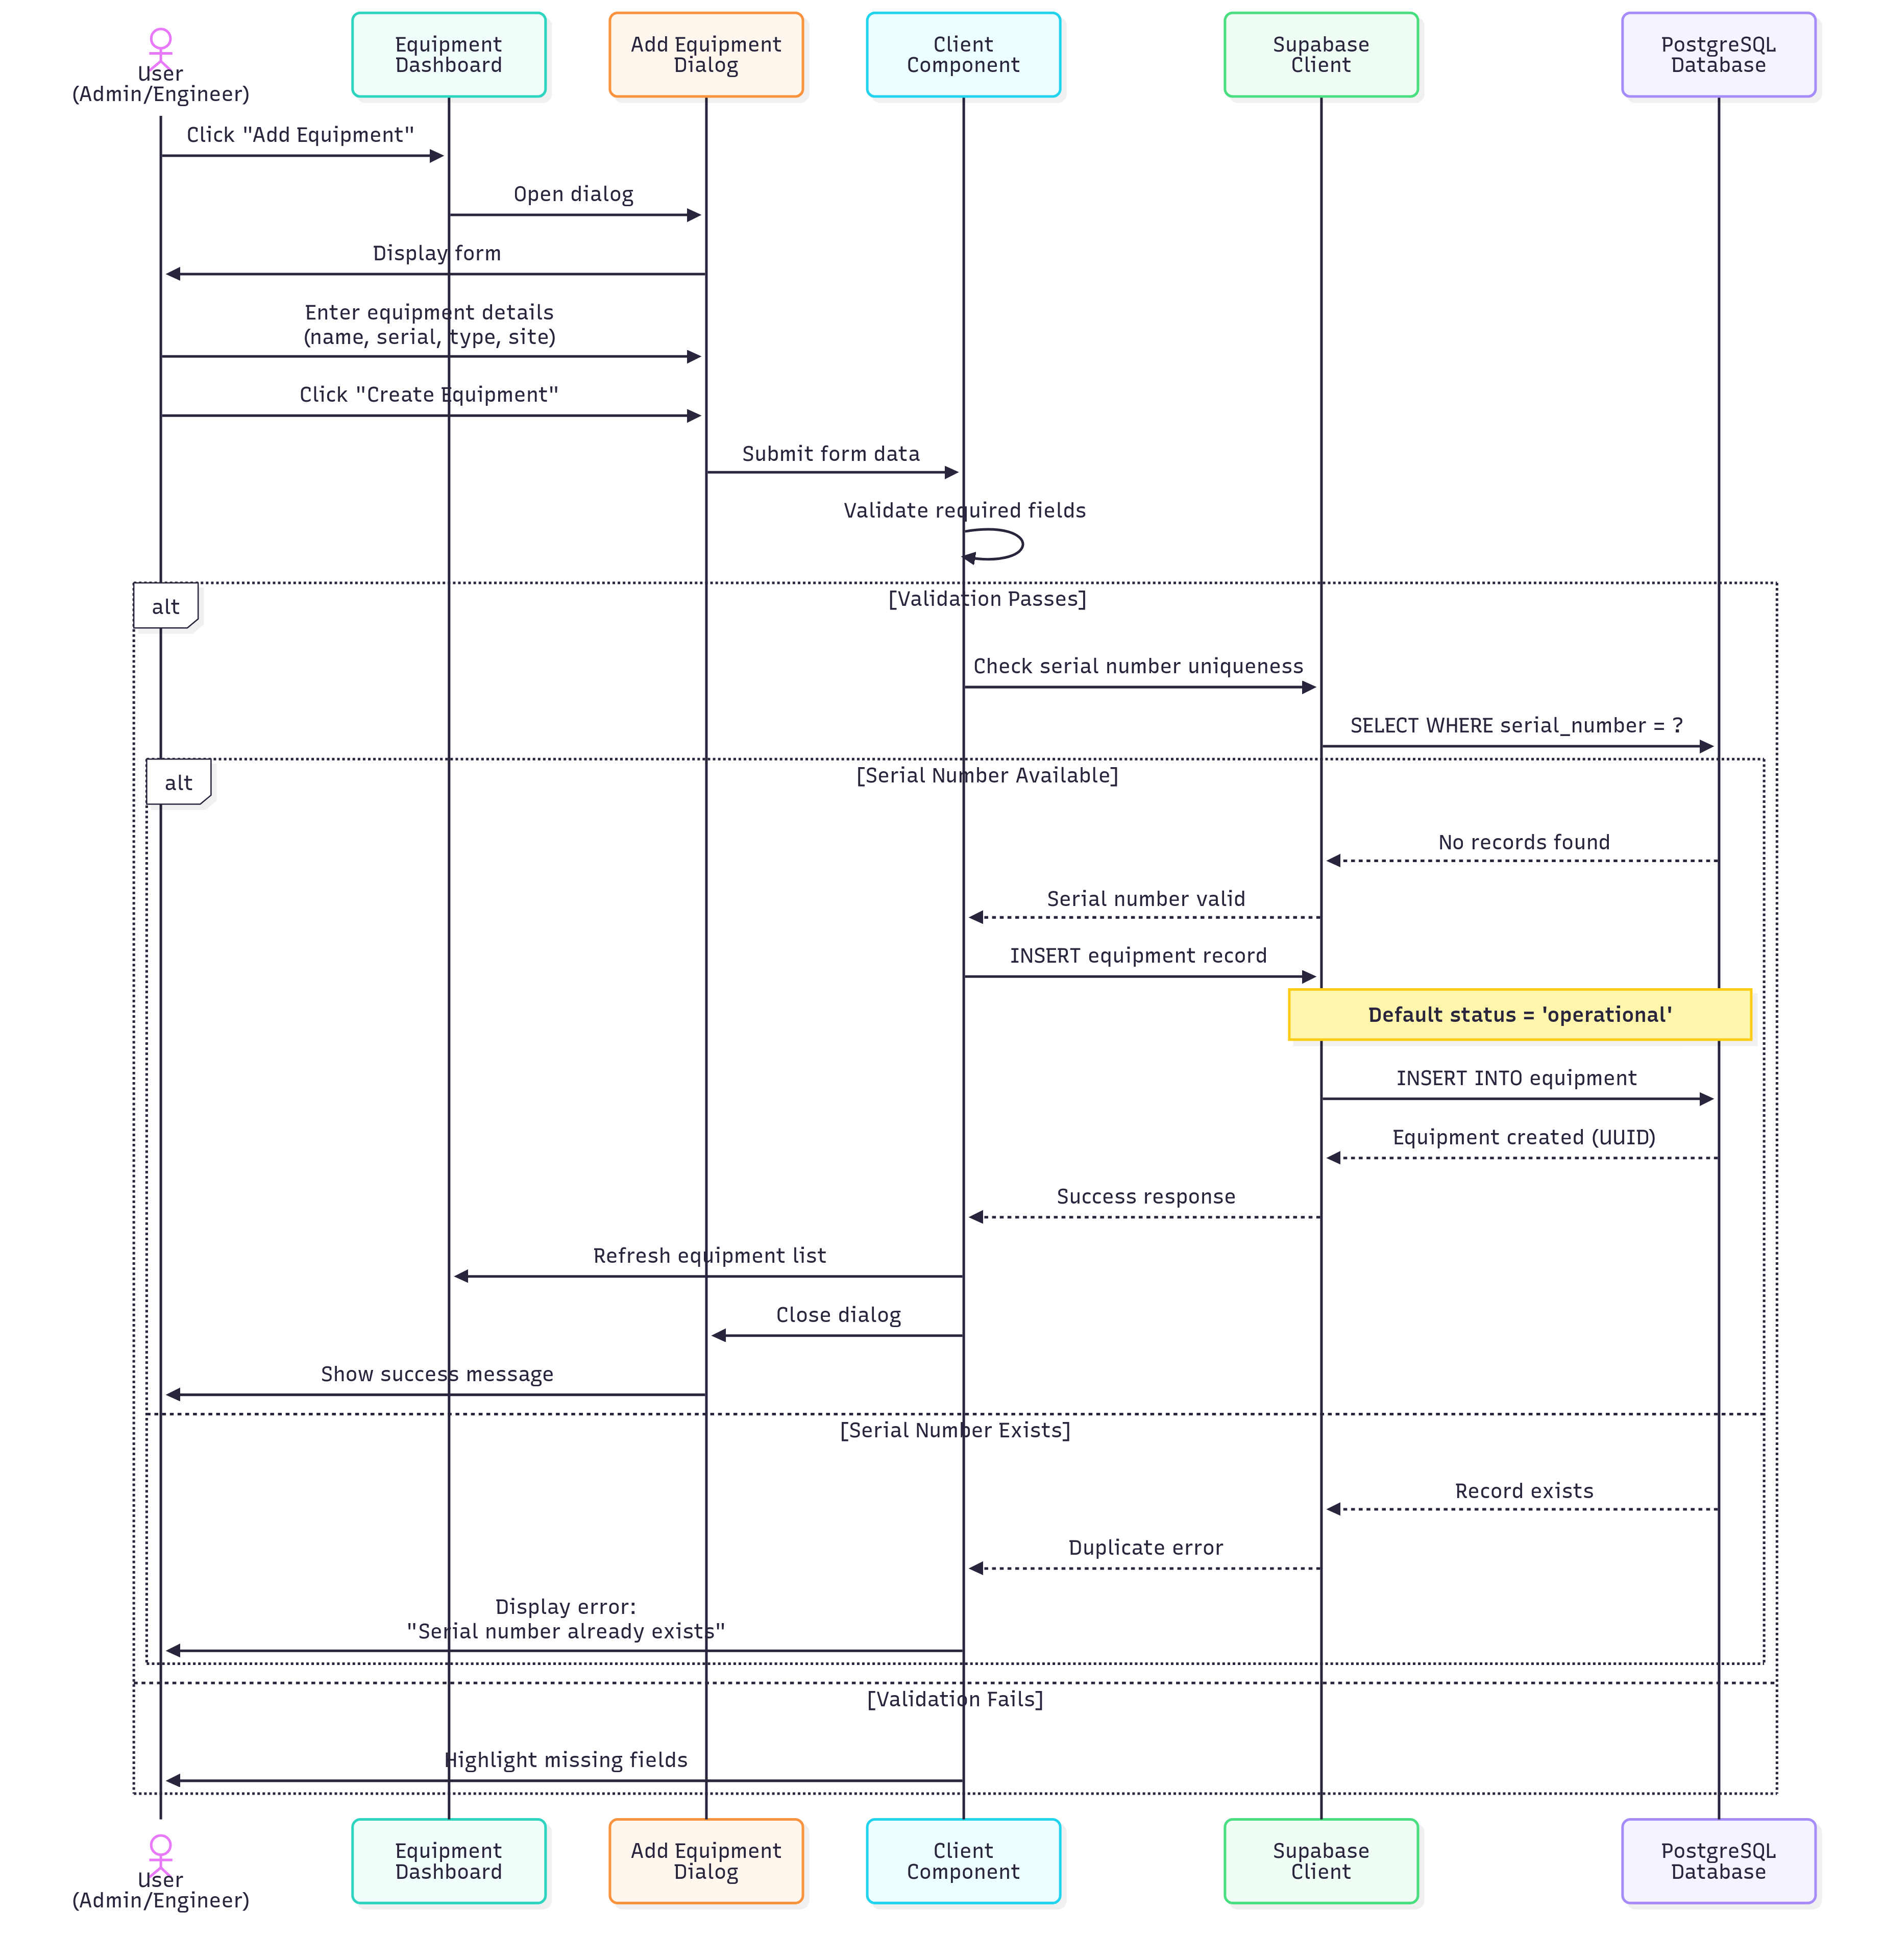
\includegraphics[width=0.95\linewidth]{img/chap_04/add_equipment_sequence.png}
    \caption{Sequence Diagram - Add Equipment Process}
    \label{fig:sequence_add_equipment}
\end{figure}

\textbf{Note on Sequence Diagram:} Following UML sequence diagram standards, return messages should use dashed arrows (-->) while request messages use solid arrows (->), clearly distinguishing between calls and responses.

The add equipment sequence (Figure 4.3) demonstrates the workflow for registering new network equipment. An authorized user (Administrator or Network Engineer) accesses the equipment management interface and clicks "Add Equipment" displaying the creation modal. After entering required details including equipment name, unique serial number, equipment type selection, brand and model information, and site assignment, the user submits the form. The validation system performs comprehensive checks on required fields and serial number format. If validation succeeds, the system queries the database to verify serial number uniqueness preventing duplicate registrations. Upon confirmation of uniqueness, the request proceeds to Supabase via \texttt{supabase.from('equipment').insert()} with Row Level Security verification ensuring only administrators and engineers can create equipment. The database assigns a UUID identifier and sets default "operational" status. Upon successful creation, the system updates the equipment list in real-time using Supabase subscriptions, closes the modal, and displays success confirmation. Duplicate serial numbers or validation failures display appropriate error messages guiding corrective action.

\subsection{Update Equipment Status Process}

Figure 4.4 illustrates the workflow for updating equipment operational state, a critical operation for field technicians reporting equipment conditions.

\begin{figure}[H]
    \centering
    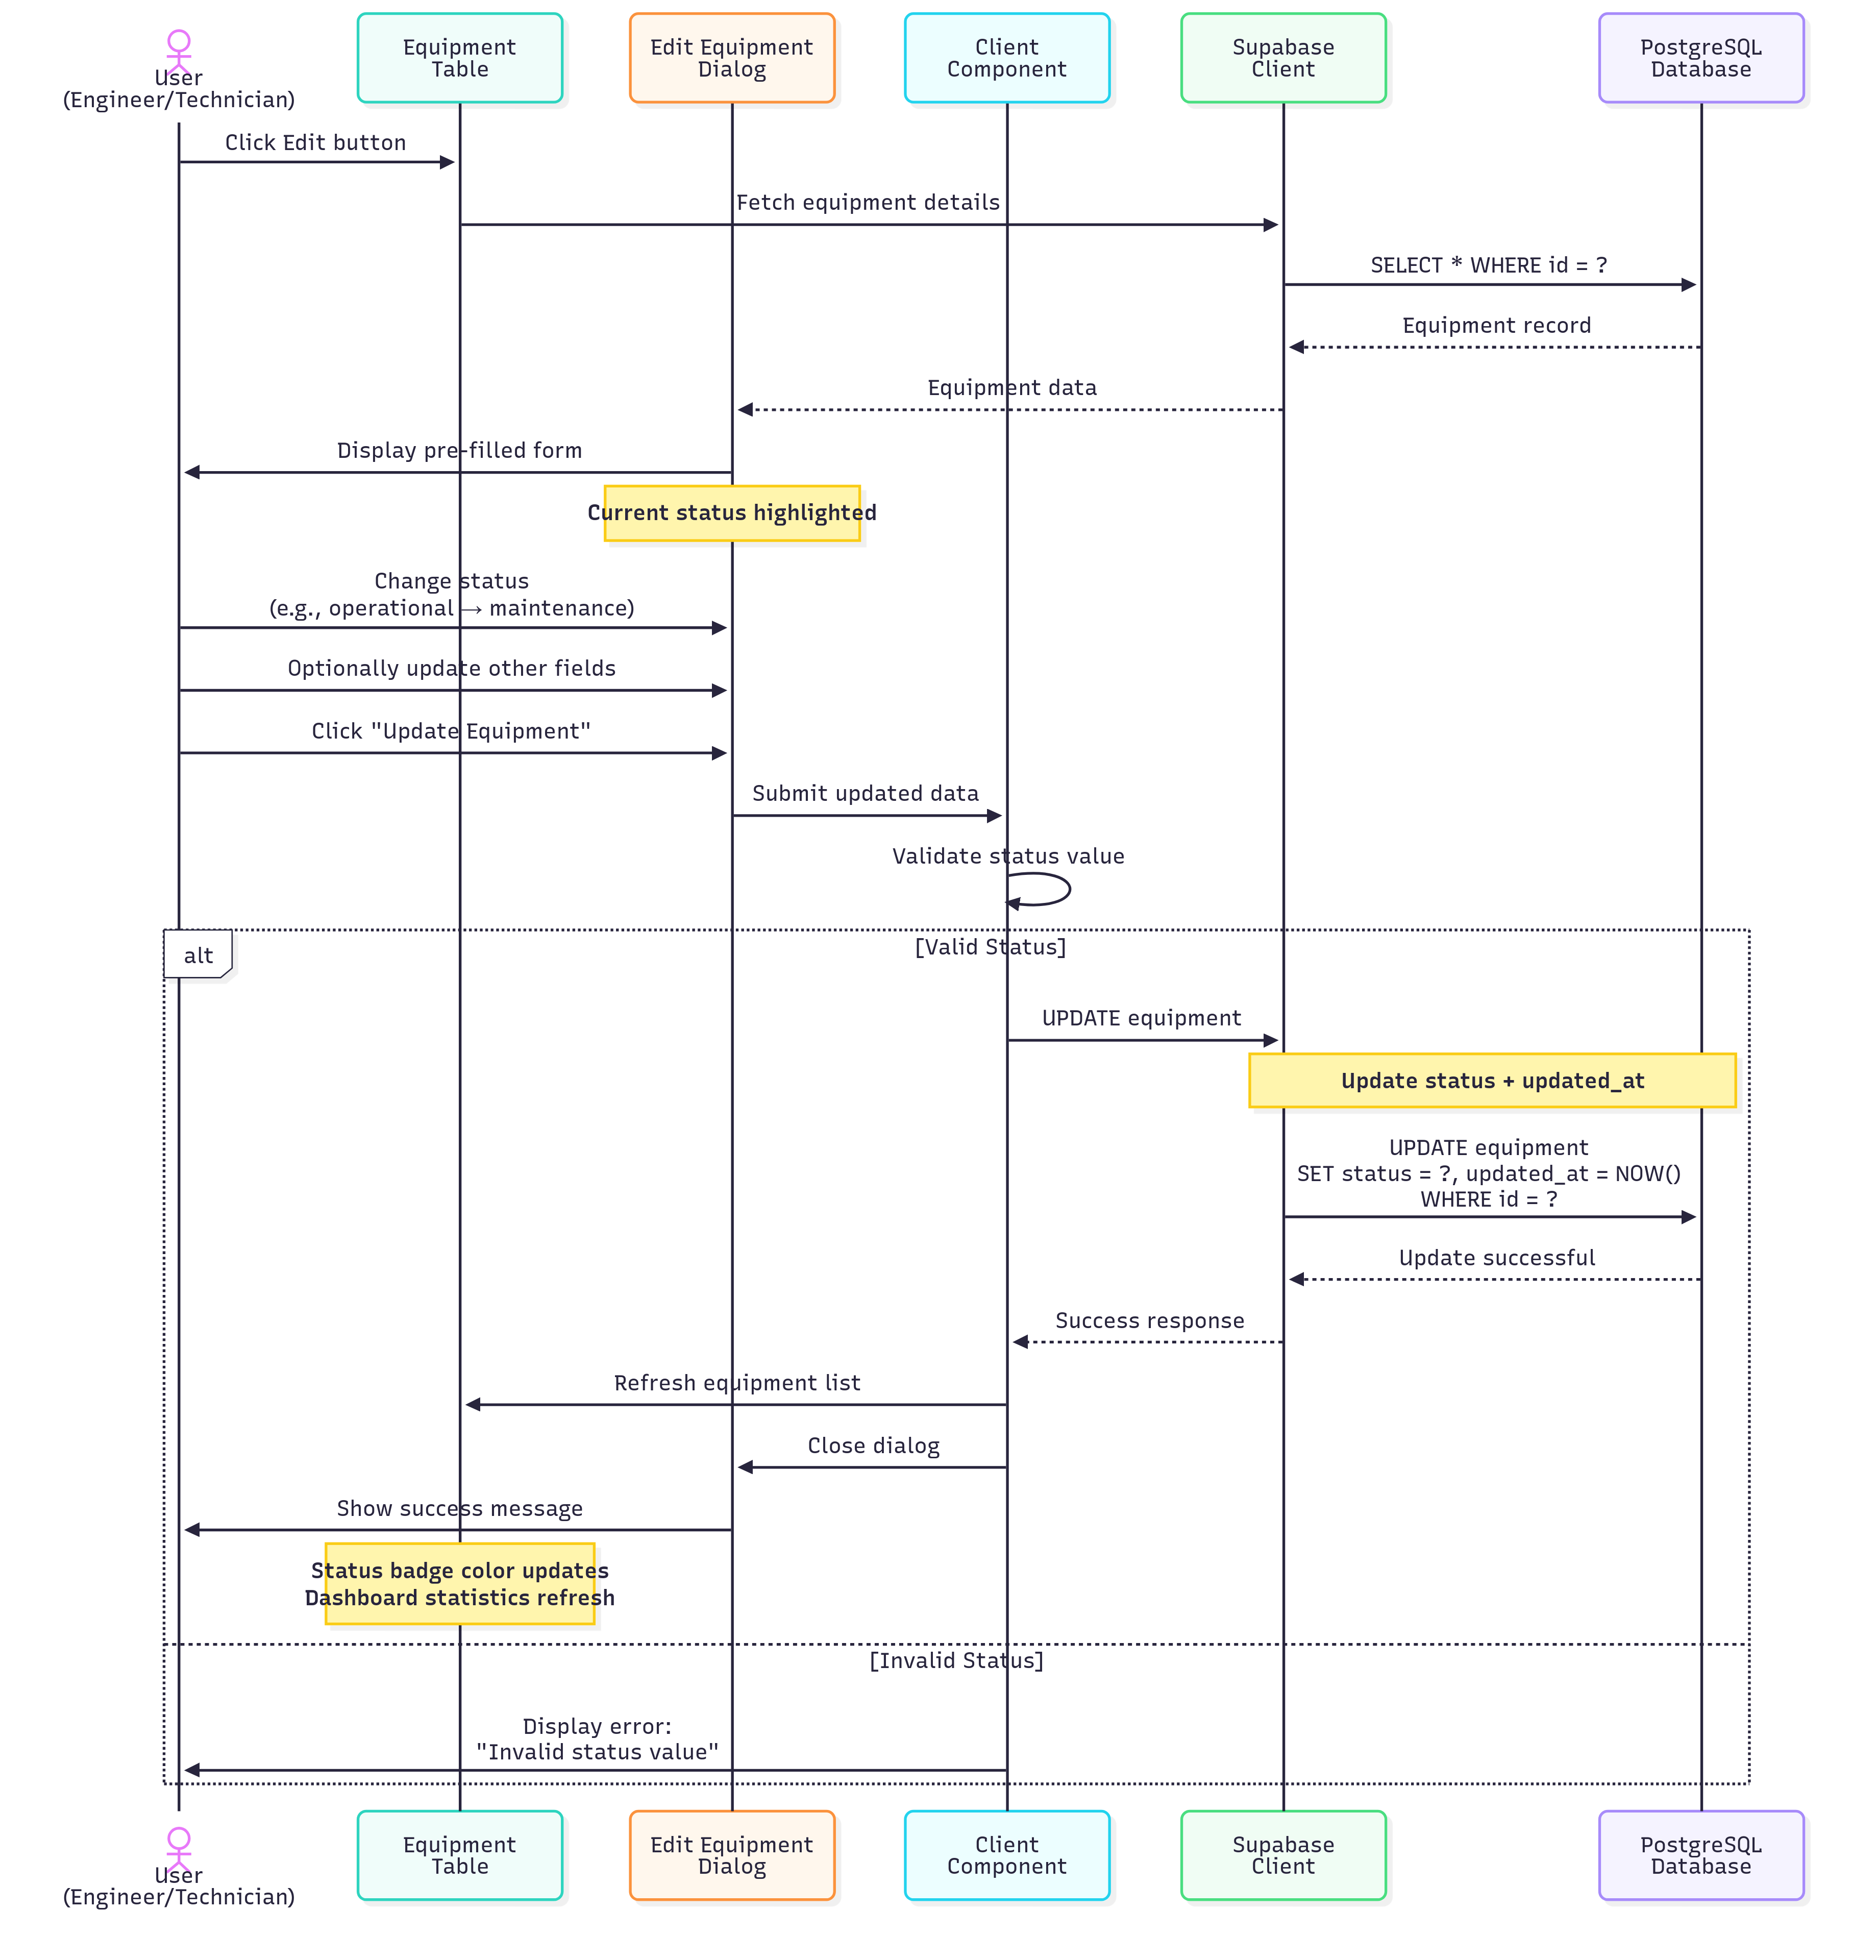
\includegraphics[width=0.95\linewidth]{img/chap_04/edit_equipment_status_sequence.png}
    \caption{Sequence Diagram - Update Equipment Status}
    \label{fig:sequence_edit_status}
\end{figure}

The equipment status update sequence (Figure 4.4) illustrates updating equipment operational state. When a user selects equipment from the list and clicks the edit status button, the system fetches current equipment details including present status value via database query. The edit dialog displays with pre-filled fields highlighting current status selection. The user modifies status selecting from valid options (operational, faulty, maintenance, offline) reflecting actual equipment condition and submits changes. The system validates the status value ensuring only defined enumeration values are accepted. Valid submissions send UPDATE request to Supabase. The database verifies user permissions through Row Level Security policies (all authenticated users can update status supporting field technician operations) and updates both status field and \texttt{updated\_at} timestamp maintaining change audit trail. Upon successful update, the equipment table refreshes across all active user sessions via real-time subscriptions, the modal closes, and dashboard statistics recalculate automatically reflecting new status distribution. Invalid status values or permission failures display appropriate error messages.

\section{Implementation}

This section presents screenshots illustrating the interfaces developed during Sprint 2 implementation.

\subsection{Equipment Dashboard}

Figure 4.5 illustrates the equipment dashboard providing operational oversight through real-time statistics.

\begin{figure}[H]
    \centering
    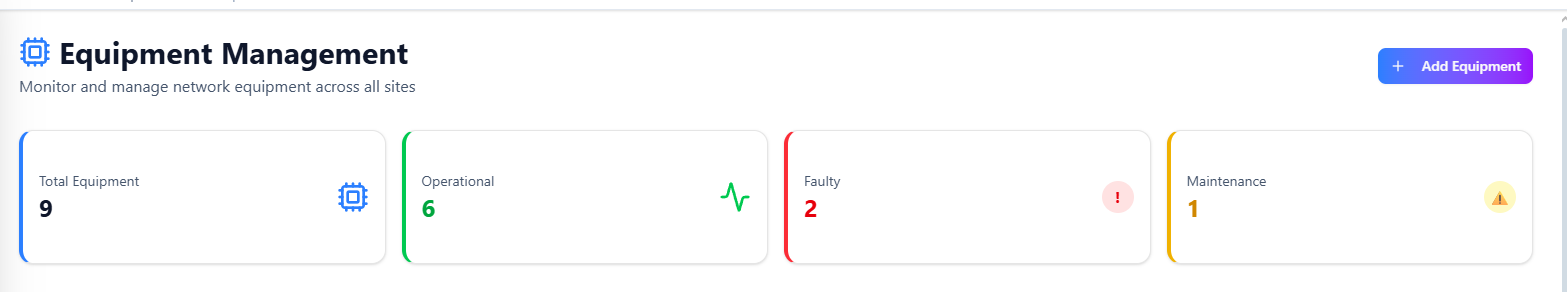
\includegraphics[width=0.9\linewidth]{img/chap_04/equipment_dashboard.png}
    \caption{Equipment Dashboard with Real-time Statistics}
    \label{fig:equipment_dashboard}
\end{figure}

The dashboard (Figure 4.5) presents four statistical cards displaying real-time equipment counts by status with color-coded visual indicators: green for operational equipment indicating healthy network assets, red for faulty equipment requiring immediate attention, yellow for equipment under maintenance showing planned service activities, and gray for offline equipment indicating powered-down or decommissioned assets. The cards update automatically when equipment status changes across the network.

\subsection{Equipment Inventory Table}

Figure 4.6 illustrates the comprehensive equipment inventory table providing complete equipment information with action controls.

\begin{figure}[H]
    \centering
    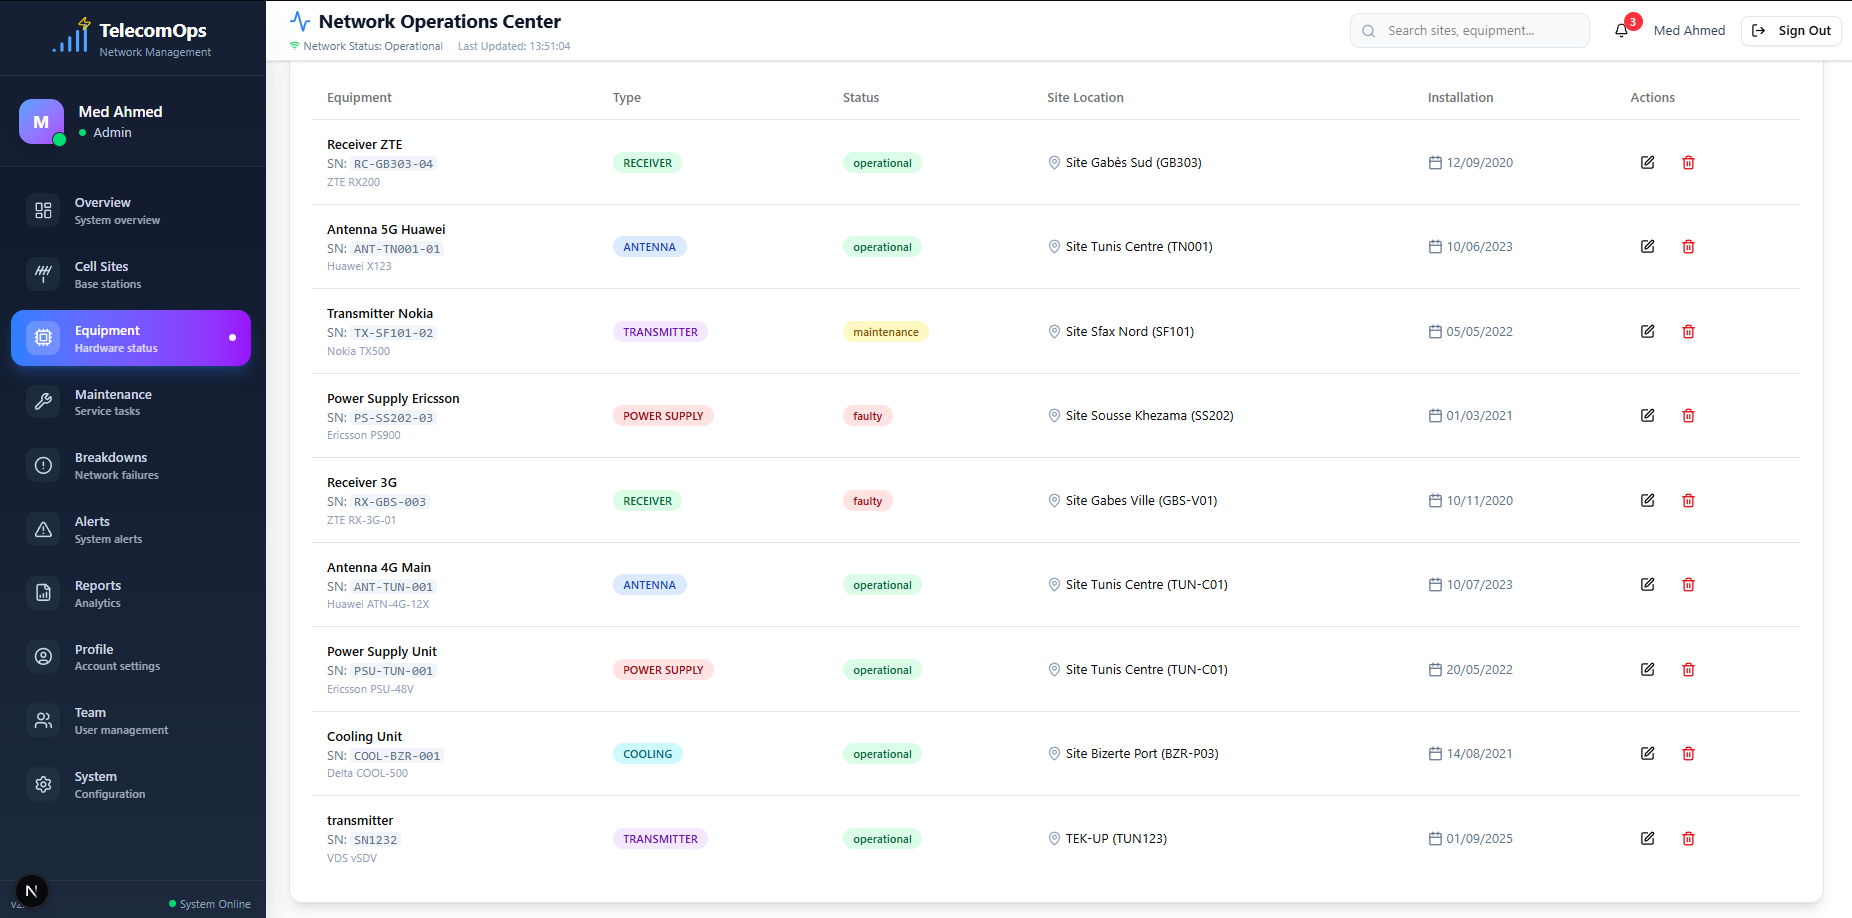
\includegraphics[width=0.9\linewidth]{img/chap_04/equipment_table.png}
    \caption{Equipment Inventory Management Table}
    \label{fig:equipment_table}
\end{figure}

The equipment table displays comprehensive information with columns for equipment name and identification, unique serial number with copy functionality, equipment type displayed as color-coded badge, operational status displayed as status badge, associated site location with hyperlink, installation date for lifecycle tracking, and action buttons (view details, edit, delete) with role-based visibility.

\subsection{Equipment Management Modals}

Figures 4.7 and 4.8 illustrate the equipment management modals implementing CRUD operations with validation and permission enforcement.

\begin{figure}[H]
    \centering
    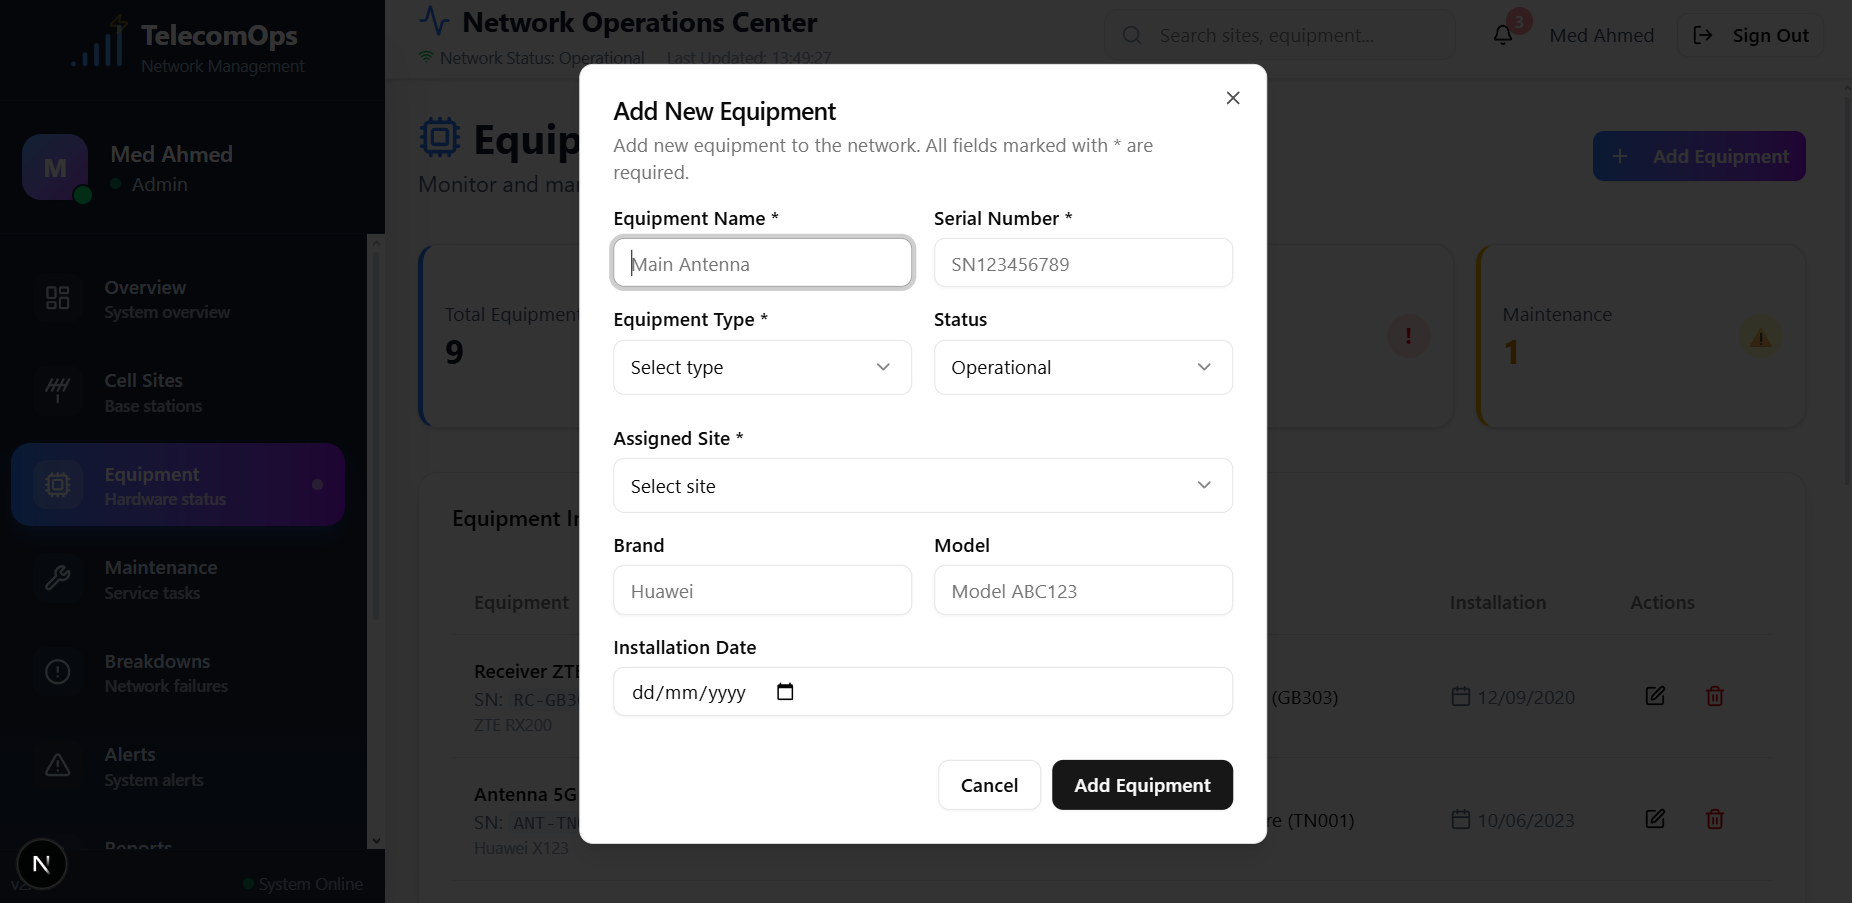
\includegraphics[width=0.9\linewidth]{img/chap_04/add_equipment_dialog.png}
    \caption{Add Equipment Modal with Validation}
    \label{fig:add_equipment_modal}
\end{figure}

\begin{figure}[H]
    \centering
    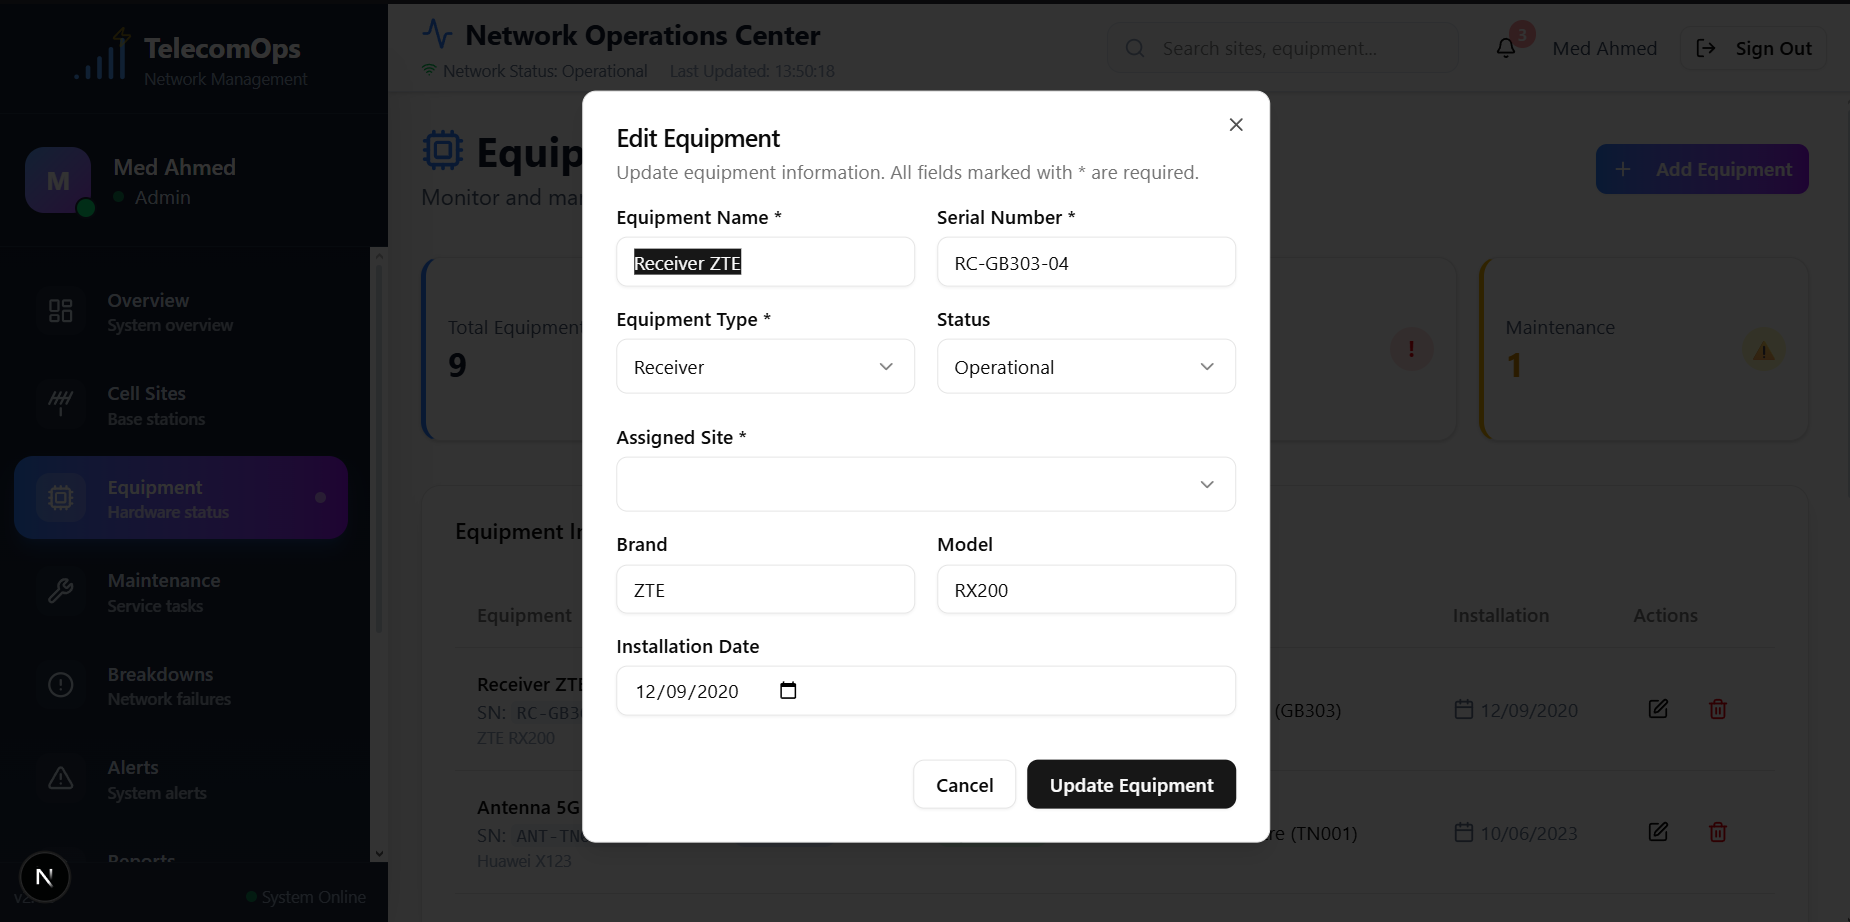
\includegraphics[width=0.9\linewidth]{img/chap_04/edit_equipment_dialog.png}
    \caption{Edit Equipment Modal with Pre-populated Data}
    \label{fig:edit_equipment_modal}
\end{figure}

The add equipment modal (Figure 4.7) implements required fields including name, serial number, equipment type, and site assignment, with optional fields for brand, model, and installation date. Serial number field includes format validation with real-time feedback. The edit equipment modal (Figure 4.8) pre-populates with current equipment information enabling selective field updates. Serial number remains immutable post-creation ensuring equipment traceability throughout lifecycle.

\section{Technical Challenges and Solutions}

Sprint 2 implementation encountered several technical challenges requiring systematic analysis and resolution.

\subsection{Serial Number Uniqueness Enforcement}

Ensuring absolute serial number uniqueness across potentially thousands of equipment items required two-tier validation approach. Client-side validation provides immediate feedback through format checking and preliminary database queries warning users before submission. Server-side enforcement through PostgreSQL unique constraint on \texttt{serial\_number} column provides absolute protection against duplicates even under concurrent creation attempts. This defense-in-depth approach addresses both user experience and data integrity requirements.

\subsection{Equipment-Site Relationship Integrity}

Maintaining referential integrity between equipment and sites while supporting site lifecycle operations required careful foreign key constraint configuration. The \texttt{site\_id} foreign key implements ON DELETE RESTRICT policy preventing site deletion when associated equipment exists. The system displays detailed warnings before site deletion attempts showing affected equipment count and requiring explicit confirmation. The NOT NULL constraint on \texttt{site\_id} ensures every equipment item maintains valid site association supporting accurate geographical equipment distribution tracking.

\subsection{Real-time Status Synchronization}

Ensuring immediate status update propagation across multiple concurrent user sessions required implementing Supabase real-time subscriptions on the equipment table. Status changes trigger automatic table re-queries for all subscribed clients, dashboard statistics recalculate automatically, and optimistic UI updates provide immediate feedback before server confirmation. This architecture supports field technician workflows where status updates must be immediately visible to network operations center personnel.

\section{Testing and Validation}

Sprint 2 underwent comprehensive testing ensuring reliability, data integrity, and proper role-based access control.

\subsection{Equipment CRUD Operations Testing}

Complete CRUD operation validation confirmed administrators perform all operations including equipment deletion, engineers create and update equipment but cannot delete ensuring operational safety, technicians view equipment and update status supporting field operations, and managers have read-only access with comprehensive statistics visibility. All unauthorized operations were properly blocked by Row Level Security policies.

\subsection{Serial Number Validation Testing}

Extensive serial number uniqueness testing included sequential duplicate attempts properly rejected with clear error messages, concurrent duplicate creation attempts from multiple sessions successfully prevented by database constraints, and serial number format validation providing immediate user feedback. Testing confirmed the two-tier validation approach provides both excellent user experience and absolute data integrity.

\subsection{Equipment Status Workflow Testing}

Equipment status transition testing verified all status changes update \texttt{updated\_at} timestamps maintaining complete audit trail, invalid status values rejected by database CHECK constraints, status modifications respect role-based permission hierarchy with appropriate error messages, and dashboard statistics recalculate correctly reflecting accurate equipment distribution across status categories.

\subsection{Performance Testing}

Performance validation confirmed equipment list queries with 1,000+ records return within 300ms meeting NFR-001 requirements, serial number uniqueness checks execute within 100ms providing responsive user experience, real-time status updates propagate to all connected clients within 1.5 seconds, and dashboard statistics calculation completes within 200ms supporting real-time operational oversight.

\section{Sprint Review and Retrospective}

Sprint 2 review with stakeholders confirmed successful delivery of all committed user stories addressing US-005A-C, US-006, and US-016A. Stakeholders particularly valued the serial number uniqueness enforcement preventing inventory confusion, real-time status updates supporting operational coordination, and hierarchical permission model reflecting organizational structure. User acceptance testing across all four user roles validated the implementation meets telecommunications asset management requirements.

The sprint retrospective identified positive outcomes including Supabase real-time subscriptions enabling seamless status synchronization, TypeScript enum types preventing invalid status values during development, and comprehensive validation providing excellent user experience. Areas for improvement include earlier stakeholder review of equipment type categories and more extensive performance testing with production-scale data volumes.

\section{Conclusion}

Sprint 2 successfully extended the TelecomOps foundation with comprehensive equipment monitoring and inventory management capabilities. The implementation delivered complete equipment CRUD operations with role-based access control, serial number uniqueness enforcement ensuring equipment traceability, real-time status monitoring supporting field operations, equipment statistics dashboards providing operational oversight, and equipment-site relationship integrity maintaining accurate asset tracking.

The sprint addressed all committed user stories (US-005A-C, US-006, US-016A) from Chapter 2's product backlog, implementing equipment inventory capabilities specified in the system architecture. The hierarchical permission model ensures appropriate access escalation from technicians through managers and engineers to administrators, reflecting the stakeholder analysis from Chapter 2.

Quality metrics exceeded established targets with successful user acceptance testing across all user roles, performance metrics surpassing NFR-001 requirements, and comprehensive validation confirming data integrity. The implementation demonstrates effective integration of Next.js, TypeScript, and Supabase while addressing real-world telecommunications asset management requirements.

Sprint 2 establishes robust equipment inventory foundation enabling subsequent features. The equipment tracking capabilities provide essential infrastructure for intervention management (Sprint 3), alert generation based on equipment status (Sprint 4), and equipment-specific analytics (Sprint 5). The unique serial number enforcement ensures equipment traceability throughout its complete lifecycle from installation through replacement.

The next chapter presents Sprint 3, titled "Breakdown Management and Intervention Planning," which leverages the site and equipment foundations to implement comprehensive fault reporting, intervention scheduling, and technician assignment capabilities, addressing user stories US-007, US-008, and US-009 from the product backlog.